\documentclass[12pt]{article}

\usepackage[a4paper]{geometry}
            
\usepackage[shortlabels]{enumitem}
\usepackage{amssymb}

\usepackage[nottoc]{tocbibind}

\usepackage{rotating}

\usepackage[square,numbers]{natbib}
\bibliographystyle{abbrvnat}



\usepackage{float}
\usepackage{blindtext}
\usepackage{enumitem} 
\usepackage{tikz}
\usepackage{tkz-berge} 
\usepackage{amsthm}
\usepackage{hyperref}
\usepackage{amsmath}
\usepackage{parskip}
\usepackage{afterpage}
\usepackage[linesnumbered,ruled,vlined]{algorithm2e}
\usepackage{algpseudocode}

\setlength{\parindent}{1em}
\setlength{\parskip}{1.3em}
\renewcommand{\baselinestretch}{1.5}


\newtheoremstyle{slplain}% name
  {2\baselineskip\@plus.5\baselineskip}% Space above
  {2\baselineskip\@plus.5\baselineskip}% Space below
  {\slshape}% Body font
  {}%Indent amount (empty = no indent, \parindent = para indent)
  {\bfseries}%  Thm head font
  {.}%       Punctuation after thm head
  { }%      Space after thm head: " " = normal interword space;
        %       \newline = linebreak
  {}%       Thm head spec


\theoremstyle{slplain}

\newtheorem{theorem}{Theorem}
\newtheorem{defi}{Definition}
\newtheorem{rema}{Remark}
\newtheorem{exam}{Example}


\title{A programming approach to vertex coloring by kernelization}

\author{{Mehri Bagherihamaneh}\\[.2cm]{317493}\\[1cm]{\small {Master thesis}}\\[.2cm]
{\small {in Mathematics}}\\[1cm]{\small {Advisor: Prof. Dr. Arie M.C.A. Koster}}\\[.5cm]{\small {Lehr-und Forschungsgebiet Diskrete Optimierung}}\\ {\small {Rheinisch-Westfaelische Technische Hochschule Aachen}}}

{\small \date{{Aachen, }\today}}


\begin{document}
 {\rmfamily 

\maketitle

\afterpage{\null\newpage}
\newpage

\begin{center}
{\bf Statutory Declaration}
\end{center}

I declare that I have developed and written the enclosed Master Thesis
completely by myself, and have not used sources or means without declaration
in the text. Any thoughts from others or literal quotations are clearly marked.
The Master Thesis was not used in the same or in a similar version to achieve
an academic grading or is being published elsewhere.

%\newline
	\end{Huge}\date{Aachen, }\today}}

\begin{flushright}
\begin{tabular}{rrr}
		&		&		& 	\hline
		&		&	 	&	    Mehri Bagherihamaneh

\end{tabular}

\end{flushright}


\afterpage{\null\newpage}
\newpage

\tableofcontents

\afterpage{\null\newpage}
\newpage
\setcounter{secnumdepth}{-2}
\begin{center}
\section{Abstract}
\end{center}
This thesis is about graph vertex coloring. The graph vertex coloring is a famous $NP$-complete combinatorial optimization problem. Recently, a new approach has been offered by using kernelization, which helps to solve vertex coloring easier with reduction of size of the  graph. In this thesis we will discuss the effect of kernelization on graphs, and reduction in size it causes, and demonstrate it by means of some sample graphs in practice. The algorithm used for coloring is "improved DSATUR-based Branch and Bound" that is an exact algorithm. Python is used as programming language. Due to its similarity with pseudo code,  Python is a good choice for these kind of works.

\afterpage{\null\newpage}
\newpage
\setcounter{secnumdepth}{2}
\section{Introduction}
Kernelization is a way to diminish size of certain problems and convert them to more manageable problems. By kernelization, a problem can be reduced to a smaller and easier problem, hence it can be solved easier and in a shorter time. 

All $NP$-hard problems above a certain size are not practically solvable. Graph vertex coloring is one such problem. In this paper, we intend to analyze how usage of kernelization can help vertex coloring in graphs which cannot be colored otherwise.

In this chapter, basic and advanced related definitions with examples for more clarification are introduced in three sections:
\begin{itemize}
\item Graph theory
\item Complexity
\item Parameterized complexity
\end{itemize}

Chapter two, describes special kernelization for vertex coloring: An algorithm by using mininmum vertex cover, an improvement for the algorithm and the theorem which proves the correctness of the algorithm.

Chapter three, describes finding minimum vertex cover through finding biggest clique in the graph.

In chapter four, one example of the algorithm from chapter three is demonstrated and prosecuted step by step.

Chapter five, investigates an exact algorithm for vertex coloring.

Chapter six, includes computational experiments and two tables of comparative results of running the Python programs for vertex coloring of some instances with and without kernelization.

The last chapter, includes some conclusions and suggestions for further works.

\newpage
\subsection{Graph Theory}
We need definitions of minimum vertex cover and biggest clique of the graph and some other notions before discussing the kernelization:


Let $G = (V, E)$ be an undirected and simple graph with $V$ and $E$, as vertex set and edge set respectively, which $|V| = n$ is the number of vertices of the graph.



\begin{defi}
An induced subgraph of a graph $G$ is another graph, which constitutes from a subset of the vertices of the graph $G$ and all of the edges connecting pairs of vertices in that subset. For $X \subseteq V(G)$, the subgraph induced by $X$ is denoted by $G[X]$ .
\end{defi}


\begin{defi}
A vertex cover $V'$ of a graph is a subset of $V$ such that for every edge $uv \in E$ , $u \in V'$ or $v \in V'$ , that means every edge has at least one endpoint in the vertex cover. 

The minimum vertex cover problem is the problem of finding a vertex  cover with minimum number of vertices in a given graph. The size of minimum vertex cover is called the vertex cover number and denoted by $\tau(G)$ .
\end{defi}

\begin{theorem}
Minimum vertex cover problem is a $NP$-complete problem.\cite{cormen} (We discuss the notion of $NP$-completeness in section \ref{comp}.) 
\end{theorem}

\begin{defi}
An independent set or stable set $S$ of a graph is a subset
of $V$ such that no two vertices of $S$ are adjacent, namely, for every two
vertices in $S$, there is no edge connecting these two vertices. 

A maximum independent set is an independent set of the largest possible size. This size is called the independence number of $G$, and denoted by $\alpha(G)$. The problem of finding maximum independent set is called the maximum independent set problem.
\end{defi}

\begin{theorem}	
Maximum independent set problem is a $NP$-hard optimization problem.\cite{karp}
\end{theorem}

\begin{rema}
A set of vertices $V'$ is a vertex cover if and only if its complement
$V \setminus V'$ is an independent set. Therefore, the number of vertices of a graph
is equal to its minimum vertex cover number, plus the size of a maximum
independent set (first proved by \href{https://en.wikipedia.org/wiki/Tibor_Gallai}{Tibor Gallai}, (1959)\cite{gallai}):

\vspace{0.5cm}
\begin{center}
$|V| = \tau(G) + \alpha(G)$
\end{center}
\end{rema}


\begin{exam}
In this graph, set $\{v_1 , v_3 , v_4 , v_6\}$ constitutes a vertex cover, but this set is not the minimum vertex cover. 

\vspace{1cm}
\begin{center}
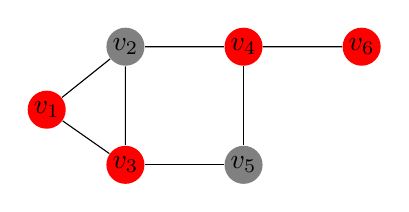
\begin{tikzpicture}
\node[circle,fill=red,inner sep=1pt,minimum size=1mm] (v1) at (0,0.2) {$v_1$};
\node[circle,fill=gray,inner sep=1pt,minimum size=1mm] (v2) at (1,1) {$v_2$};
\node[circle,fill=red,inner sep=1pt,minimum size=1mm] (v3) at (1,-0.5) {$v_3$};
\node[circle,fill=red,inner sep=1pt,minimum size=1mm] (v4) at (2.5,1) {$v_4$};
\node[circle,fill=gray,inner sep=1pt,minimum size=1mm] (v5) at (2.5,-0.5) {$v_5$};
\node[circle,fill=red,inner sep=1pt,minimum size=1mm] (v6) at (4,1) {$v_6$};

\draw (v1)--(v2)--(v4)--(v6);
\draw (v1)--(v3)--(v2);
\draw (v3)--(v5)--(v4);
\end{tikzpicture}

\end{center}

As can be seen, the subset $\{v_2 , v_3 , v_4\}$ is a minimum vertex cover (red) and $\{v_1 , v_5 , v_6\}$ is a maximum independent set (blue).

\vspace{1cm}
\begin{center}
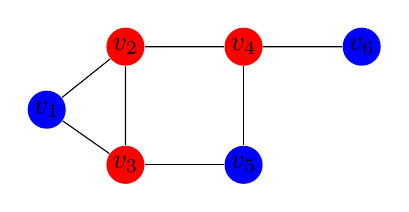
\begin{tikzpicture}
\node[circle,fill=blue,inner sep=1pt,minimum size=1mm] (v1) at (7,0.2) {$v_1$};
\node[circle,fill=red,inner sep=1pt,minimum size=1mm] (v2) at (8,1) {$v_2$};
\node[circle,fill=red,inner sep=1pt,minimum size=1mm] (v3) at (8,-0.5) {$v_3$};
\node[circle,fill=red,inner sep=1pt,minimum size=1mm] (v4) at (9.5,1) {$v_4$};
\node[circle,fill=blue,inner sep=1pt,minimum size=1mm] (v5) at (9.5,-0.5) {$v_5$};
\node[circle,fill=blue,inner sep=1pt,minimum size=1mm] (v6) at (11,1) {$v_6$};

\draw (v1)--(v2)--(v4)--(v6);
\draw (v1)--(v3)--(v2);
\draw (v3)--(v5)--(v4);
\end{tikzpicture}
\end{center}
\end{exam}

\begin{defi}
A clique in a graph is a subset of vertices such that every two distinct vertices are adjacent. 

A maximal clique is a clique that cannot be extended by adding one more adjacent vertex. The maximal clique problem is the problem of finding all maximal cliques in a graph.
% and it may require exponential time as there exist graphs with exponentially many maximal cliques. For example in a complete graph %with $2n$ vertives, there are $2^n$ maximal cliques.
%(Take the complete graph on $2n$ nodes and remove a perfect matching there are $2^n$ maximal cliques.) 

A maximum clique is a clique that has the maximum possible number of vertices. The clique number, $\omega(G)$, is the number of vertices in a maximum clique of $G$. 
\end{defi}

\begin{theorem}
In general, the problem of finding the maximum clique for a given graph is $NP$-hard\cite{karp}.
\end{theorem}

\begin{exam}
The graph shown has one maximum clique, the triangle $\{v_1 , v_2 , v_3\}$, and four more maximal cliques, the pairs 
$\{v_2 , v_4\}$ , $\{v_3 , v_5\}$ , $\{v_4 , v_5\}$ , $\{v_4 , v_6\}$.
\vspace{1cm}
\begin{center}
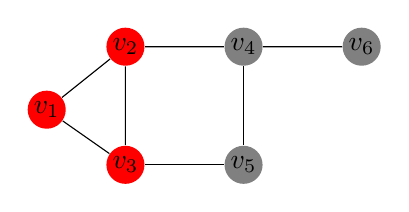
\begin{tikzpicture}
\node[circle,fill=red,inner sep=1pt,minimum size=1mm] (v1) at (0,0.2) {$v_1$};
\node[circle,fill=red,inner sep=1pt,minimum size=1mm] (v2) at (1,1) {$v_2$};
\node[circle,fill=red,inner sep=1pt,minimum size=1mm] (v3) at (1,-0.5) {$v_3$};
\node[circle,fill=gray,inner sep=1pt,minimum size=1mm] (v4) at (2.5,1) {$v_4$};
\node[circle,fill=gray,inner sep=1pt,minimum size=1mm] (v5) at (2.5,-0.5) {$v_5$};
\node[circle,fill=gray,inner sep=1pt,minimum size=1mm] (v6) at (4,1) {$v_6$};

\draw (v1)--(v2)--(v4)--(v6);
\draw (v1)--(v3)--(v2);
\draw (v3)--(v5)--(v4);
\end{tikzpicture}
\end{center}
\end{exam}

\begin{defi}
A vertex coloring is an assignment of labels or colors to each
vertex of a graph such that no edge connects two vertices with the same color.

The chromatic number of a graph is the smallest number of colors needed for
vertex coloring and denoted by $\chi(G)$. 

A vertex coloring of a graph with $k$ or fewer colors is known as a $k$-coloring. A proper $k$-coloring is an assignment of $k$ colors to the vertices of a graph so that no two adjacent vertices have the same color. 

A proper $k$-coloring of a graph $G$ can be shown as a function $f: V(G) \to \{1, 2, 3, . . . , k\}$ such that adjacent vertices get different colors, namely in a proper coloring, for all edges $\{u, v\}$ we have $f(u) \not= f(v)$.
\end{defi}


\begin{exam}
The petersen graph is $3$-colorable as shown:
\vspace{1cm}
\begin{center}
\begin{tikzpicture}[rotate=90]
  \GraphInit[vstyle=Hasse]
  \SetVertexNoLabel \SetUpVertex[MinSize=2pt] \grPetersen[RA=2,RB=1]
  \SetUpVertex[inner sep=1pt,MinSize=2pt]
  \AddVertexColor{red}{a0,b1,b2,a3}
  \AddVertexColor{green}{a1,b0,a4}
  \AddVertexColor{blue}{b4,b3,a2}
\end{tikzpicture}
\end{center}

\end{exam}
\vspace{0.5cm}

\newpage
\subsection{Complexity}{\label{comp}}

\begin{defi}
For an instance $I$ from instance set $\mathcal{I}$, a decision problem $\Pi$ is a YES-NO question which asks if
there is at least one solution for the problem $\Pi$ in $I$.
\end{defi}

\begin{exam}
An example of a decision problem is CLIQUE problem: For a graph $G$ and an integer $k$, does there exist at least one clique of size $k$ in the graph? 
\end{exam}

\begin{theorem}
CLIQUE problem is $NP$-complete. \cite{karp}
\end{theorem}

\begin{exam}
$k$-COLORING is a decision problem, which asks if we can color a graph $G$ with $k\in\mathbb{N}$ or fewer colors. For $k \geq 3$ in general graphs, $k$-COLORING is $NP$-complete. We discuss it in chapter \ref{dsat}.
\end{exam}

\begin{exam}
Another example of a decision problem is VERTEX COVER: For a graph $G$ and an integer $k$, is there any vertex cover of size at most $k$ in the graph? 
\end{exam}

\begin{theorem}
VERTEX COVER problem is $NP$-complete. \cite{karp}
\end{theorem}

\begin{defi}
In computational complexity theory, there are some different classes of decision problems:

\begin{itemize}
\item Fundamental complexity class $P$ (PTIME), contains all decision problems that can be solved by a deterministic \href{https://en.wikipedia.org/wiki/Turing_machine}{Turing machine}\cite{turing} in a polynomial time. 

Many natural problems are in $P$. For example the problem of determining if a number is prime, is in $P$\cite{manindra}.

\item $NP$ (for non-deterministic polynomial) is a complexity class that contains all decision problems for which the instances where the answer is "yes" have efficiently verifiable proofs by deterministic computations that can be performed in polynomial time. $P\subset NP$.

\item $NP$-hard class includes the problems like $H$ such that every problem $M$ in class $NP$ can be reduced in polynomial time to $H$. Informally, $NP$-hard class contains the hardest problems in $NP$. 

With this definition, it is obvious that, if $P \not= NP$, $NP$-hard problems cannot be solved in polynomial time. An example of a $NP$-hard example is the traveling salesman problem.\cite{lawler}

\item $NP$-complete class is equal to the intersection of the $NP$ class and $NP$-hard class, namely, A decision problem $L$ is $NP$-complete if satisfies these two conditions:
\begin{enumerate}
\item Every problem in $NP$ is reducible to $L$ in polynomial time that means $L$ is $NP$-hard.

\item $L$ is in $NP$.
\end{enumerate}
\end{itemize}
\end{defi}

\begin{defi}
A propositional logic (boolean) formula is constructed by some variables (atomic formulas) and constants using operators AND (conjunction "$\land$"), OR (disjunction "$\lor$"), NOT (negation "$\lnot$") and parentheses. 

Every variable can get logical values (TRUE or FALSE). 

A literal is an atomic formula (atom) or its negation. 

A clause is an expression constructed from a finite  disjunction or conjunction of literals.
\end{edfi}

\begin{exam}
Some examples for boolean formulas are:

\begin{itemize}
\item $x_1 \land (x_2 \lor\lnot x_1)$, where $(x_2 \lor\lnot x_1)$ is a clause.
\item $(A \land B) \lor \lnot(B \lor C)$
\item $X_1 \lor (\lnot X_2 \lor X_3) $
\end{itemize}
\end{exam}

\begin{defi}
A boolean formula is satisfiable if it can be TRUE by assigning logical values to its variables. 
\end{defi}

\begin{exam}
One example of satisfiable formulas:

\begin{center}
 $\varphi = d\lor (a\land b\land (c\lor d \land\lnot a))$
\end{center}

For verifying, we don't need to check all possibilities. It is enough to find one answer (T for TRUE and F for FALSE):

\begin{table}[H]
\begin{center}
\begin{tabular}{c|c|c|c|c}
$a$ & $b$ & $c$ & $d$ & $\varphi$\\
\hline
F & F & F & T & T\\ 
&&&&\\
&&&&\\
\end{tabular}
\end{center}
\end{table}
\end{exam}

\begin{exam}
One example of unsatisfiable formulas:

\begin{center}
$\theta = X \land \lnot X$
\end{center}

For each value for $X$, the formula is FALSE:

\begin{table}[H]
\begin{center}
\begin{tabular}{c|c|c}
$X$ & $\lnot X$ & $\theta$\\
\hline
T & F & F \\ 
F & T & F\\
\end{tabular}
\end{center}
\end{table}
\end{exam}
\end{exam}


\begin{defi}
A boolean formula is in conjunctive normal form (CNF) if it is a conjunction of one or more disjunctions of variables.
\end{defi}

\begin{exam}
These formulas are in CNF form.
\begin{itemize}
\item $\lnot x \land (y \lor z)$
\item $x_1 \lor x_2$
\item $x_1 \land x_2$
\end{itemize}
\end{exam}

\begin{defi}
For a given CNF formula $\varphi$, the boolean satisfiability problem (SAT) is a decision problem which asks whether the formula $\varphi$ is satisfiable. The $3$-SAT problem is a SAT problem with at most $3$ variables in each clause. 
\end{defi}

\begin{theorem}\label{3-sat}
The $3$-SAT problem is $NP$-complete. \cite{cook}
\end{theorem}

The following problem is an unsolved problem in computer science:

Is $P = NP$ or $P \not= NP$? This question is equivalent to this one: 

If correctness of the solution to a problem is easy to check, is the problem easy to solve? 

Some scientists believe that $P = NP$ and some don't. These two cases are shown in figure \ref{fig}.

%\vspace{2cm}
\newcommand{\boundellipse}[3]% center, xdim, ydim
{(#1) ellipse (#2 and #3)
}

\begin{figure}[!ht]
\centering


\begin{tikzpicture}
\draw (0,0) circle (1.5cm);
\draw \boundellipse{0,-0.75}{1.1}{0.75};
\draw (-1.5,3) .. controls (-1,0) and (1,0) .. (1.5,3);
\node at (0,2) {\tiny $NP$-Hard};
\node at (0,1.2) {\tiny $NP$-Complete};
\node at (-1,0) {\tiny $NP$};
\node at (0,-0.75) {\tiny $P$};
\node at (0,-2) {\tiny $P \not= NP$};
\node at (4,1) [label={[rotate=90]{\tiny complexity}}];
\draw[->] (4,-2) -- (4,4);
\draw (8,0) circle (1.5cm);

\draw (6.5,2) .. controls (5.40,-2.7) and (10.6,-2.7) .. (9.5,2);
\node at (8,2) {\tiny $NP$-Hard};
\node at (8,0) {\tiny $NP$-Complete = $P$ = $NP$};

\node at (8,-2) {\tiny $P = NP$};
\end{tikzpicture}
\caption{\tiny Euler diagram for $P$, $NP$, $NP$-hard and $NP$-complete set of problems}\label{fig}
\end{figure}

\newpage
\subsection{Parameterized Complexity}

If we assume $P \not = NP$, there are some problems with exponential running time when complexity is measured in terms of the input size only, but they are computable in a time that is polynomial in the input size and exponential in a parameter $k$. Hence, for small parameter (but large instance), we can use efficient exact algorithms. 

\begin{defi}
A parameterized problem is a pair $(\Pi, \kappa)$ in which $\Pi$ is a
decision problem with instance set $\mathcal{I}$ and $\kappa : \mathcal{I} \to \mathbb{N}$, which is a polynomial
time computable function, called parameter.
\end{defi}

\begin{exam}
An example of a parameterized problem is parameterized-vertex cover, denoted $k$-VERTEX COVER:

Input : graph $G = (V, E)$ and a number $k \in \mathbb{N}$

parameter : $k$

problem : Is there any vertex cover set in $G$ with maximum size of $k$?
\end{exam}



\newpage

\section{Kernelization}

Kernelization is a method to build efficient polynomial-time algorithms, 
in which the size of the given problem instance is reduced to an equivalent smaller instance which is called kernel. 

In this case, size of the kernel (new input) just depends on the parameter and not on the original input size. 

Actually, kernelization or data reduction is helpful in practical computer implementation related to $NP$-hard problems. After kernelization, a slower exact algorithm can be used for solving the new smaller instance (kernel).

\begin{defi}
Let $(\Pi, \kappa)$ be a parameterized problem, $I\in\mathcal{I}$ an instance and $\kappa: \mathcal{I} \to \mathbb{N}$ a parameterization for $\Pi$:

A polynomial time computable function $f : \mathcal{I} \times \mathbb{N} \to \mathcal{I} \times \mathbb{N}$ is called a
kernelization for $(\Pi, \kappa)$ , if $f(I, \kappa(I)) = (I', \kappa(I'))$ such that it satisfies these 3 properties:

\begin{enumerate}[(i)]
\item For each $I \in \mathcal{I}$, $(I, \kappa(I))$ is a "YES"-instance of $\Pi$ iff $(I', \kappa(I'))$ is a "YES"-instance of $\Pi$.

\item There is a function $f': \mathbb{N} \to \mathbb{N}$, such that $|I'| \leq f'(\kappa(I))$

\item $\kappa(I')\leq \kappa(I)$.
\end{enumerate}

$I'$ is kernel of $(\Pi, \kappa)$ and $f'(\kappa(I))$ is called the size of the kernel.

\end{defi}




We can often find a kernel in polynomial time, hence we have an algorithm for the original problem whose running time is the sum of the time needed for kernelization step (polynomial time) and the time to solve the kernel (non-polynomial but bounded by the parameter).

\vspace{1cm}
\begin{exam}
An example of a kernelization algorithm is the kernelization of
the vertex cover problem by S. Buss and J. Goldsmith\cite{buss}. 

The input is graph $G$ and a positive integer 
$k$ and the output is a vertex cover set with at most size $k$ if any exists, or
a failure exception if no such set exists. This problem is $NP$-hard. 

These reduction rules are used to kernelize the problem:

\begin{enumerate}
\item For a given instance $(G,k)$ of the problem, if $v$ is an isolated vertex of $G$, remove it. An isolated vertex $v$ cannot cover any edges, so $v$ is not contained in any minimal cover. The new instance is $(G - v , k)$.


\item If $G$ contains a vertex $v$ of degree greater than $k$, each vertex cover with size at most $k$ should contain $v$, since otherwise all of its neighbors (more than $k$ vertices) should be in the vertex cover to cover the incident edges. Then $v$ will be picked for optimal vertex cover. Remove such a $v$ from the graph and decrease $k$ by one. 
The new instance is $(G - v , k - 1)$.

\item If neither of the previous two rules can be applied anymore, and the graph still has more than $k^2$ edges, then the graph cannot contain a vertex cover of size $k$, because, after eliminating all vertices of degree greater than
$k$, each remaining vertex can only cover at most $k$ edges and a set of
$k$ vertices could only cover at most $k^2$ edges. In this case, the instance
may be replaced by an instance with two vertices, one edge, and $k = 0$,
which also has no solution.
\end{enumerate}

After applying these rules repeatedly until no more reductions are applicable, a kernel that has at most $k^2$ edges and at most $2k^2$ vertices will be obtained, because each edge has at most two endpoints and there are no isolated vertices.

All reduction rules (kernelization) are trivially applicable in linear time. After kernelization, the vertex cover problem may be solved by a brute force search algorithm that tests whether each subset of the kernel is a vertex cover of the kernel. Thus, the vertex cover problem can be solved in time $\mathcal{O}(2^{2k^2} + |V| + |E|)$ which is efficiently solvable for small $k$.
\end{exam}

In this thesis, we are interested in a kernelization on vertex coloring. 
A kernelization on $3$-coloring using vertex cover has been discussed in \href{https://onedrive.live.com/view.aspx?resid=D39E73028C0B20E6!2586&ithint=file%2cpptx&app=PowerPoint&authkey=!AFs8zyWC8bfQ0PA}{a presentation} by Bart. Jansen, (Bonn, 2016) \cite{bart}.

Steps of the algorithm are:

\begin{enumerate}
\item Compute $2$-approximate vertex cover $X$

\item $\forall S\subseteq X$ of size $3$
\begin{itemize}
\item Mark a common neighbor of $S$
\end{itemize}
\item Delete all unmarked $v \not\in X$

\item Output resulting $G'$ on $n'$ vertices:

\begin{center}
$n' \leq |X| + |X|^3 \leq 2k + (2k)^3$
\end{center}
\end{enumerate}

$G$ is $3$-colorable iff $G'$ is $3$-colorable. Run time for the algorithm is $\mathcal{O}(min|X|^3)$.

the algorithm and correctness proof can be generalized to $q$-COLORING. \cite{kra}


by substituting $3$ with $q$ in the recent algorithm:

\begin{theorem}{\label{main theorem}}
$G$ is $q$-colorable iff $G'$ is $q$-colorable. Run time for the algorithm
is $\mathcal{O}(min|X|^q)$.
\end{theorem}

\begin{proof}
Let $G$ be a graph and $X$ with $|X| = k$ be it's vertex cover. Create an
equivalent instance $G'$ as follows: At first, let be $G' = G[X]$,  the subgraph induced by $X$. 

For each subset
$S \subseteq X$ of size $q$, mark a common neighbor of $S$ if there is such a vertex.
Then delete all unmarked vertices out of $X$ . After that, add marked vertices to $G'$. 

Proof of the equivalency: From a proper $q$-coloring $f'$ of $G'$ we
can extract a proper partial $q$-coloring $f$ of $G[X]$ and $f$ can be extended to the rest of $G$, otherwise, there is a vertex in $G \setminus X$ whose neighbors have all $q$ colors, and then this vertex is a common neighbor of a subset of size $q$ from
$X$ and hence is also in $G'$ contradicting that $f'$ is proper.

Now, we represent the instance $G'$ in $\mathcal{O}(|X|^q) = \mathcal{O}(k^q)$ bits as follows: Store 
adjacency matrix of $G'[X]$ in exactly $k^2$ bits. Then for each subset $S$ of $X$ 
of size $q$ (they are less than $k^q$) store exactly one bit for specifying whether 
there is or there is not a vertex that is a common neighbor of vertices in $S$. The 
run time of the algorithm is less than $k^2 + k^q$, and it concludes the proof.
\end{proof}
\vspace{1cm}

At first I tried to implement the algorithm in the presentation, exactly following steps as stated in the presentation, but it was too slow, because of high number of subsets of vertex cover, specially with larg graphs. In this way, kernelization took much more time than coloring of the original graph itself. Then to optimize the execution time, I considered the problem from the other side. 

In this new aspect, we don't need to compute all subsets of the vertex cover of size $3$ or in general $q$, which is too slow. Instead, we consider the nodes outside of the vertex cover and for each, we check if it has $3$ ($q$) distinct vertices in the vertex cover. This version yields the same result as the original algorithm. (Algorithm \ref{kern})

\vspace{1cm}

\begin{algorithm}[H]
\SetAlgoLined
\DontPrintSemicolon
  \caption{Kernelization of vertex coloring by using vertex cover}{\label{kern}}

Find exact minimum vertex cover\;

Iterate all vertices outside of vertex cover\;

If the vertex has $3$ distinct neighbors in vertex cover and it wasn't
visited yet, then mark it\;

Delete all unmarked vertices outside of vertex cover\;
\end{algorithm}

\newpage

On the other hand, by finding exact minimal vertex cover instead of $2$-approximation for it, we have a smaller vertex cover, hence the number of its subsets of a specific size will be reduced, therefore there will be more vertex outside of vertex cover and then more unmarked vertices which will be deleted. This results in a smaller kernel which is more satisfiable.


The next step is improving vertex cover which will be discussed in the next chapter.






\newpage
\section{Minimum Vertex Cover}{\label{vertex_cover}}
Minimum vertex cover is a typical example of an $NP$-complete optimization problem that has an approximation algorithm. We are interested in an exact solution; one way to solve the problem is integer linear programming.

\begin{defi}
Linear programming (LP) is an optimization problem with linear objective function (a linear mathematical model) and result based on some set of linear equality and inequality constraints. 

LP is a modeling technique in mathematics to find maximum (or minimum) of a linear function on a convex polytope (optimize). In fact, this convex polytope is presentation of some inequality constraints on variables of the function. The solution for a linear programming is a point in the polytope where this function has the largest (or smallest) value if such a point exists.

Canonical form of expression for linear program is:

\begin{align*}
&optimize \; \;\; \;\;\; c^Tx\\
&subject\; to \;\;\; \;\; Ax \leq b\\
&and	\qquad\qquad	 x \geq 0
\end{align*}

where $A$ is a matrix of coefficients, $(.)^T$ is the matrix transpose, $x$ is the vector of variables (to be found), $c$ and $b$ are vectors of coefficients.

The maximize (minimize) expression called the objective fuction and the inequalities are constraints.

Joseph Fourier (French, 1768-1830) was the first person who published in 1827 a method for solving a system of linear inequalities. \cite{gerard}

Linear programming in which variables may take only integer values, is known as integer linear programming (ILP), namely, in constraints, instead of $x\geq 0$, in ILP we have $x\in \mathbb{Z}$.
\end{defi}


Consider this formulation for vertex cover by integer linear programming (ILP), where for each vertex $v$ we have a variable $X_v$, which $X_v = 1$ if $v$ is in the vertex cover and $X_v = 0$ if $v$ is not chosen to be in the vertex cover:

\begin{align*}
&minimize \; \;\; \; \sum_{v\in V}X_v \qquad\qquad\quad (minimize \; the \; number \;  of \;  vertices \; in \; vertex \; cover)\\
&subject\; to \;\;\; \; X_u + X_v  \geq 1 , \qquad (cover \; every \; edge \; of \; the \; graph)\\
&\qquad 	\qquad\qquad\qquad	 \forall \{u,v\} \in E\\
&and	\qquad\qquad	 \forall v, X_v\in \{0,1\} \quad (every \; vertex \; is \; in \; the \; vertex \; cover \; or \; not)
\end{align*}

This model will work well for small instances, but might be troublesome for some larger instances. ILP formulation can be improved  by restricting to valid inequalities.\cite{Gerard2} 

In this case, there is a class of valid inequalities of interest: clique inequalities.

If there is a clique in the graph, it is easy to verify that at least all but one
of its vertices should be included in the vertex cover. So, this requirement can be modeled as a linear constraint.

For the best result, we can restrict this ILP to maximal cliques inequality:


\begin{align*}
&minimize \; \;\; \; \sum_{v\in V}X_v\\
&subject\; to \;\;\; \; X_u + X_v  \geq 1 ,\\
&\qquad 	\qquad\qquad\qquad	 \forall \{u,v\} \in E\\
&and	\qquad\quad\;\; \sum_{v\in K_n}x_v \geq n - 1\\
& \qquad\qquad \qquad\qquad for\; every\; maximal\; clique\; K_n\; in\; the\; graph\\
&and	\qquad\qquad	 \forall v, X_v\in \{0,1\}
\end{align*}

Every edge is also a clique, and hence, the edge inequality can be removed
while including the clique inequalities:

\begin{align*}
&minimize \; \;\; \; \sum_{v\in V}X_v\\
&subject\; to \;\;\; \; \sum_{v\in K_n}x_v \geq n - 1\\
& \qquad\qquad \qquad\qquad for\; every\; maximal\; clique\; K_n\; in\; the\; graph\\
&and	\qquad\qquad	 \forall v, X_v\in \{0,1\}
\end{align*}

There is a good algorithm for finding maximal cliques of a graph, called Bron-Kerbosch\cite{bron} algorithm. It is a recursive  backtracking algorithm. In algorithm \ref{bron} we see three given sets $R$, $P$ and $X$. At first the sets $R$ and $X$ are empty and $P$ is vertex set of the graph. The algorithm finds the maximal cliques which include all of vertices of $R$, some vertices in $P$, and none vertices from $X$. In each recursive call, $P$ and $X$ have no intersection, but their union constructs the cliques which will be added to $R$. The process continues untill $P$ and $X$ are empty and the output will be the set $R$. This algorithm is efficient in worst-case. For given graph $G$ with $n$ vertex, $G$ has at most $3^{n/3}$ maximal cliques and the worst-case running time of the algorithm is $\mathcal{O}(3^{n/3})$ \cite{moon}. 


It is used in this thesis by means of function \href{https://networkx.github.io/documentation/networkx-1.10/reference/generated/networkx.algorithms.clique.find_cliques.html}{find cliques} from NetworkX library of python:

\newpage

\begin{algorithm}\label{bron}
\begin{algorithmic}

\Function{BronKerbosch}{$R, P, X$}{

        \If{$P$ and $X$ are both empty}{
        
		  	 report $R$ as a maximal clique\\	
		 }\EndIf
		\For{vertex $v$ in $P$}{
		
			   BronKerbosch$(R \cup \{v\}, P \cap N(v), X \cap N(v))$
			   
			    $P := P\setminus \{v\}$
			    
			   	   $X := X\cup \{v\}$\\
		}\EndFor
}\EndFunction
\end{algorithmic}
\caption{Bron-Kerbosch}
\end{algorithm}


\newpage


Next step is making a model with AMPL\cite{ampl} for vertex cover restricted by
maximal cliques, and solving it with CPLEX\cite{cplex} for some samples.

AMPL (A Mathematical Programming Language) is an algebraic modeling language to describe and solve high-complexity problems for large-scale mathematical computing. 

One advantage of AMPL is the similarity of its syntax to the mathematical notation of optimization problems.

CPLEX (IBM ILOG CPLEX Optimization Studio) is an optimization software package developed by \href{https://www.ibm.com/us-en/}{IBM company} \cite{IBM}. It is a good solver for AMPL.

Maximal cliques will be obtained using a Python program and written in a data file 
with vertices and edges of graph. This data file is used to compute vertex cover by solving AMPL model with CPLEX as a solver.

The obtained vertex cover is used in another program to compute the
kernel and then coloring the graph, which will be discussed in chapter \ref{dsat}.
\newpage
AMPL model for vertex cover restricted to maximal cliques

\hline

\begin{verbatim}
# Declarations
set V;
set E within V cross V;
set Idx;
set Q within Idx cross V;
set cnt within Idx cross V;
var x {v in V} binary;
# integrality constraints.
# Objective Function
minimize cover_size: sum { v in V } x[v];
# Constraints
subject to clique {c in Idx}:
sum {(a, b) in Q: a = c} x[b] >= card{(a,b) in Q: a = c} -1;
\end{verbatim}

\newpage


\section{An Example}{\label{section}}
In this section, for better explanation we prosecute the instructions of kernelization 
step by step for $M_4 = \mu(M_3)$ graph, the third graph of \href{https://en.wikipedia.org/wiki/Mycielskian}{Mycielski graphs} \cite{mycielski}.
%\href{http://mat.gsia.cmu.edu/COLOR/instances/myciel3.col}{instance "myciel3.col"} from DIMACS instances\cite{instance}:

This graph has $11$ vertices and $20$ edges and is known to be $4$-colorable:

\vspace{1cm}

\begin{center}
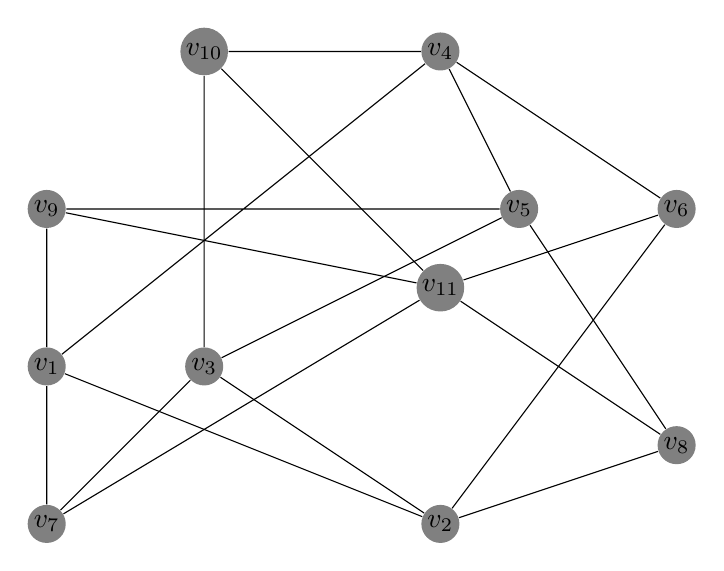
\begin{tikzpicture}
\node[circle,fill=gray,inner sep=1pt,minimum size=1mm] (v1) at (0,0) {$v_1$};
\node[circle,fill=gray,inner sep=1pt,minimum size=1mm] (v2) at (5,-2) {$v_2$};
\node[circle,fill=gray,inner sep=1pt,minimum size=1mm] (v3) at (2,0) {$v_3$};
\node[circle,fill=gray,inner sep=1pt,minimum size=1mm] (v4) at (5,4) {$v_4$};
\node[circle,fill=gray,inner sep=1pt,minimum size=1mm] (v5) at (6,2) {$v_5$};
\node[circle,fill=gray,inner sep=1pt,minimum size=1mm] (v6) at (8,2) {$v_6$};
\node[circle,fill=gray,inner sep=1pt,minimum size=1mm] (v7) at (0,-2) {$v_7$};
\node[circle,fill=gray,inner sep=1pt,minimum size=1mm] (v8) at (8,-1) {$v_8$};
\node[circle,fill=gray,inner sep=1pt,minimum size=1mm] (v9) at (0,2) {$v_9$};
\node[circle,fill=gray,inner sep=1pt,minimum size=1mm] (v10) at (2,4) {$v_{10}$};
\node[circle,fill=gray,inner sep=1pt,minimum size=1mm] (v11) at (5,1) {$v_{11}$};


\draw (v4)--(v1)--(v2)--(v3)--(v5)--(v9)--(v1);
\draw (v1)--(v7)--(v3)--(v10)--(v4)--(v6)--(v2)--(v8)--(v11);
\draw (v7)--(v11)--(v10);
\draw (v9)--(v11)--(v6);
\draw (v4)--(v5)--(v8);
\end{tikzpicture}
\end{center}

\vspace{1cm}

Step 1. Find exact minimum vertex cover:

First of all, the program finds the biggest clique on it. It has no clique with size more than $2$.

The input data file for AMPL contains these lines:
\newpage
{\small 
\begin{verbatim}
set Q := (0 , *) 1 , 9
(1 , *) 1 , 2
(2 , *) 1 , 4
(3 , *) 1 , 7
(4 , *) 2 , 8
(5 , *) 2 , 3
(6 , *) 2 , 6
(7 , *) 3 , 10
(8 , *) 3 , 5
(9 , *) 3 , 7
(10 , *) 4 , 10
(11 , *) 4 , 5
(12 , *) 4 , 6
(13 , *) 5 , 8
(14 , *) 5 , 9
(15 , *) 11 , 8
(16 , *) 11 , 9
(17 , *) 11 , 10
(18 , *) 11 , 6
(19 , *) 11 , 7;
set V := 1,2,3,4,5,6,7,8,9,10,11;
set E := (1, 9),(1, 2),(1, 4),(1, 7),(2, 8),(2, 3),(2, 6),(3, 10),(3, 5),
(3, 7),(4, 10),(4, 5),(4, 6),(5, 8),(5, 9),(6, 11),(7, 11),(8, 11),(9, 11),
(10, 11);
set Idx := 0,1,2,3,4,5,6,7,8,9,10,11,12,13,14,15,16,17,18,19;
set cnt := (1, 2),(12, 2),(3, 2),(13, 2),(8, 2),(15, 2),(18, 2),(9, 2),
(11, 2),(16, 2),(17, 2),(19, 2),(6, 2),(2, 2),(4, 2),(14, 2),(5, 2),(0, 2),
(7, 2),(10, 2);
\end{verbatim}
}
Where $Q$ is the set of cliques of the graph, which contains 20 cliques of size $2$.

After that, its minimum vertex cover will be computed with AMPL using the solver CPLEX. The output file contains:

\noindent 1 \\
2 \\
3 \\
4 \\
5 \\
11 \\

Then, the set $X = \{v_1 , v_2 , v_3 , v_4 , v_5 , v_{11}\}$  (shown below in red) is the minimum vertex cover, while the $2$-approximate vertex cover is $Y = \{v_1 , v_2 , v_3 , v_4 , v_5 , v_6 , v_8 , v_9 , v_{10} , v_{11}\}$.

\vspace{1cm}

\begin{center}
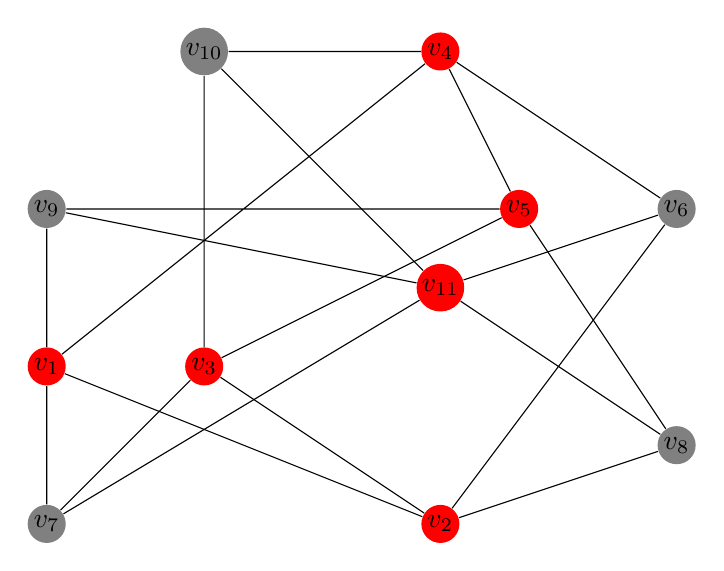
\begin{tikzpicture}
\node[circle,fill=red,inner sep=1pt,minimum size=1mm] (v1) at (0,0) {$v_1$};
\node[circle,fill=red,inner sep=1pt,minimum size=1mm] (v2) at (5,-2) {$v_2$};
\node[circle,fill=red,inner sep=1pt,minimum size=1mm] (v3) at (2,0) {$v_3$};
\node[circle,fill=red,inner sep=1pt,minimum size=1mm] (v4) at (5,4) {$v_4$};
\node[circle,fill=red,inner sep=1pt,minimum size=1mm] (v5) at (6,2) {$v_5$};
\node[circle,fill=gray,inner sep=1pt,minimum size=1mm] (v6) at (8,2) {$v_6$};
\node[circle,fill=gray,inner sep=1pt,minimum size=1mm] (v7) at (0,-2) {$v_7$};
\node[circle,fill=gray,inner sep=1pt,minimum size=1mm] (v8) at (8,-1) {$v_8$};
\node[circle,fill=gray,inner sep=1pt,minimum size=1mm] (v9) at (0,2) {$v_9$};
\node[circle,fill=gray,inner sep=1pt,minimum size=1mm] (v10) at (2,4) {$v_{10}$};
\node[circle,fill=red,inner sep=1pt,minimum size=1mm] (v11) at (5,1) {$v_{11}$};


\draw (v4)--(v1)--(v2)--(v3)--(v5)--(v9)--(v1);
\draw (v1)--(v7)--(v3)--(v10)--(v4)--(v6)--(v2)--(v8)--(v11);
\draw (v7)--(v11)--(v10);
\draw (v9)--(v11)--(v6);
\draw (v4)--(v5)--(v8);
\end{tikzpicture}
\end{center}

\vspace{1cm}

Step 2. Iterate all vertices outside of vertex cover:

The vertices outside of vertex cover are $\{v_6, v_7, v_8, v_9, v_{10}\}$

Step 3. If the vertex has $q$ distinct neighbors in vertex cover and it wasn't visited yet, then mark it:
\begin{enumerate}
\item For $q = 4$ and the vertex cover $X$, 
\begin{itemize}

\item $v_6$ has no $4$ neighbors in $X$.

\item $v_7$, $v_8$, $v_9$ and $v_{10}$ have no $4$ neighbors in $X$, either. 
\end{itemize}

Then no vertices will be marked.

Step 4. Delete all unmarked vertices outside of the vertex cover:

All of the vertices out of $X$ are unmarked and will be removed. Then the output(kernel) is the set
$\{v_1 , v_2 , v_3 , v_4 , v_5 , v_{11}\}$:


\vspace{1cm}

\begin{center}
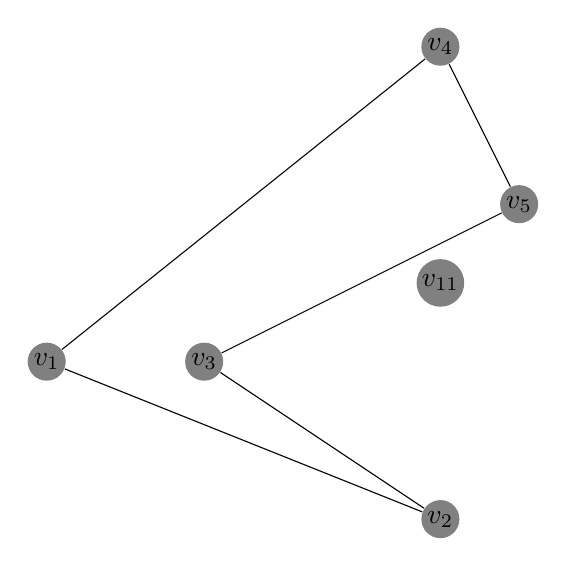
\begin{tikzpicture}
\node[circle,fill=gray,inner sep=1pt,minimum size=1mm] (v1) at (0,0) {$v_1$};
\node[circle,fill=gray,inner sep=1pt,minimum size=1mm] (v2) at (5,-2) {$v_2$};
\node[circle,fill=gray,inner sep=1pt,minimum size=1mm] (v3) at (2,0) {$v_3$};
\node[circle,fill=gray,inner sep=1pt,minimum size=1mm] (v4) at (5,4) {$v_4$};
\node[circle,fill=gray,inner sep=1pt,minimum size=1mm] (v5) at (6,2) {$v_5$};
\node[circle,fill=gray,inner sep=1pt,minimum size=1mm] (v11) at (5,1) {$v_{11}$};


\draw (v4)--(v1)--(v2)--(v3)--(v5);
\draw (v4)--(v5);
\end{tikzpicture}
\end{center}
\vspace{1cm}

This kernel can be colored with $3$ and therefore with $4$ colors.

\vspace{1cm}

\begin{center}
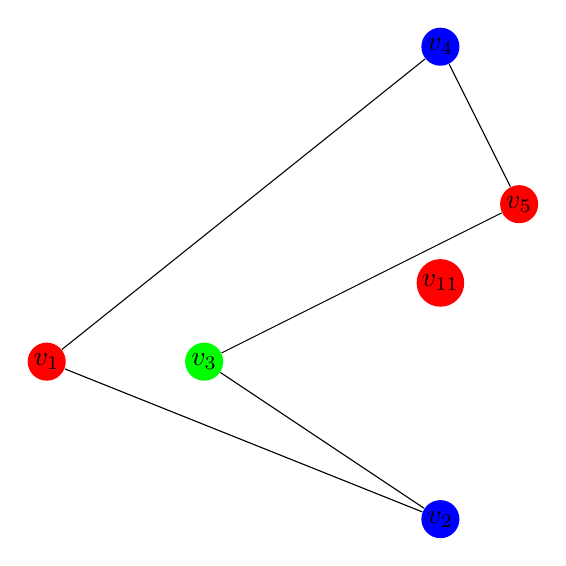
\begin{tikzpicture}
\node[circle,fill=red,inner sep=1pt,minimum size=1mm] (v1) at (0,0) {$v_1$};
\node[circle,fill=blue,inner sep=1pt,minimum size=1mm] (v2) at (5,-2) {$v_2$};
\node[circle,fill=green,inner sep=1pt,minimum size=1mm] (v3) at (2,0) {$v_3$};
\node[circle,fill=blue,inner sep=1pt,minimum size=1mm] (v4) at (5,4) {$v_4$};
\node[circle,fill=red,inner sep=1pt,minimum size=1mm] (v5) at (6,2) {$v_5$};
\node[circle,fill=red,inner sep=1pt,minimum size=1mm] (v11) at (5,1) {$v_{11}$};


\draw (v4)--(v1)--(v2)--(v3)--(v5);
\draw (v4)--(v5);
\end{tikzpicture}
\end{center}
\vspace{1cm}


If we consider set $Y$ as vertex cover, then only vertex $v_7$ is out of $Y$ and it doesn't have 4 neighbors in $Y$, hence no 
vertex will be marked and just $v_7$ will be removed, then the kernel is the set 
$\{v_1 , v_2 , v_3 , v_4 , v_5 , v_6 , v_8 , v_9 , v_{10} , v_{11}\}$ which is not as good, due to bigger kernel size.

\item For $q = 3$, and the vertex cover $X$,
\end{enumerate}

\begin{itemize}
\item $v_6$ has these four neighbors: $\{v_4 , v_2 , v_{11}\}$

\item $v_7$ has these four neighbors: $\{v_1 , v_3 , v_{11}\}$

\item $v_8$ has these four neighbors: $\{v_2 , v_5 , v_{11}\}$ 

\item $v_9$ has these four neighbors: $\{v_1 , v_5 , v_{11}\}$

\item $v_{10}$ has these four neighbors: $\{v_4 , v_3 , v_{11}\}$ 
\end{itemize}

Mark these vertices: $\{v_6, v_7, v_8, v_9, v_{10}\}$.


Now, there is no unmarked vertex out of $X$,

Step 4. Delete all unmarked vertices outside of the vertex cover:
 
hence the kernel is equal to the original graph and is $4$-colorable.

If we consider set $Y$ as the vertex cover, then only vertex $v_7$ is out of $Y$ and it doesn't have 4 neighbors in $Y$ , hence there is no unmarked vertex out of $Y$, hence the kernel is equal to the original graph.
\end{itemize}

\newpage

\section{DSATUR}{\label{dsat}}
Graph coloring for general graphs has $NP$-complete complexity:
\vspace{-0.5cm}
\begin{theorem}
$k$-COLORING for $k \geq 3$ is $NP$-complete. \cite{karp}
\end{theorem}
\vspace{-1cm}
\begin{proof}
\vspace{-0.5cm}
Sketch of proof:

To prove this theorem, it is enough to prove it for $k = 3$; because if it could be solved in polynomial time for arbitrary $k$, then it could also be solved in polynomial time for $k=3$: L\'aszl\'o Lov\'asz has proved $k$-COLORABILITY reduces to $3$-COLORABILITY. \cite{Laszlo}

As discussed in section \ref{comp}, we need to prove both of these:
\begin{itemize}
\item $3$-COLORING is in $NP$ class
\item It is $NP$-hard. 
\end{itemize}

A given $3$-coloring can be easily validated in linear time by any means of traversing the graph (DFS or BFS) and keeping track of end point colors, hence $3$-COLORING is in $NP$.  

For prove of $NP$-hardness, a reduction from $3$-SAT \cite{karp} is used. In order to reduction, we need to construct a graph $G_\varphi$ correspondence to a $3$-CNF formula $\varphi$ with $n$ variables $t_1, t_2,\dots, t_n$ and $m$ clauses. We should prove $G_\varphi$ is $3$-colorable iff $\varphi$ is satisfiable.


We omit the rest of the proof here.

\end{proof}

DSATUR is one of several heuristic algorithms which try to find the best possible solution by ordering nodes properly before the greedy search. The Greedy coloring method is the simplest algorithm which takes an ordering of nodes of a graph and colors these with the smallest possible color.

At first, one definition is needed:

\begin{defi}
Let $G$ be a simple and partially colored graph. The saturation degree of a vertex is the number of different colors to which it is adjacent (colored vertices).\cite{brelaz}
\end{defi}

In DSATUR algorithm (from {\bf d}egree {\bf sat}uration), nodes with higher degree of saturation are picked first, this yields a specific ordering of nodes for backtracking.

\vspace{1cm}

\begin{algorithm}[H]
\SetAlgoLined
\DontPrintSemicolon
  \caption{DSATUR (so called because it uses saturation degree)\cite{brelaz}}

  Arrange the vertices by decreasing order of degrees.\;
   Color a vertex of maximal degree with color $1$.\;
  Choose a vertex with a maximal saturation degree. If there is an
equality, break the tie by choosing any vertex of maximal degree in the uncolored
subgraph.\;
    Color the chosen vertex with the least possible (lowest numbered)
color.\;
  If all the vertices are colored, stop. Otherwise, return to step 3.\;
 
\end{algorithm}

\newpage

DSATUR algorithm in its original form is not an exact algorithm and not much useful for our purpose in this paper. 

There are several inhancements and variation, all based on DSATUR. One of them is "DSATUR-based Branch-$\&$-Bound" which gives an exact solution, optimized by node ordering proposed by DSATUR. This algorithm is used in this thesis.

If the vertices are being colored successively with the least possible color in a
given order, the coloration is started from a clique. (lower bounds on the 
chromatic number.)

In exact algorithm, in first step we begin to color with the biggest clique in the DSATUR algorithm.



\newpage
\newgeometry{left=1in,right=1.2in,top=1in,bottom=1in}
\begin{algorithm}[H]
\SetAlgoLined
\DontPrintSemicolon
  \caption{Randall-Brown's Modified Algorithm\cite{randall}}
  
{\small  Find a maximal clique $K$. Let dimension of clique is $w$. By using DSATUR
beginning with this clique, find an initial coloration with $r$ colors (an
upper bound) and a rank (coloration) order of the vertices. If $w = r$ , stop.\\

 Color the vertices of the clique $K$ with $1, 2, . . . w$ successively. For each
vertex $v$ in $G$ let $U(v) \in \{1, 2, . . . r + 1\}$ is the set of colors which can color
$v$. For each vertex $x_k$ out of the clique, let $U(x_k) = U(x_k) - j$ where $j$ is
the color of a vertex in $K$ which is adjacent to $x_k$.\\

 Let $k = w + 1$ and $q = r$.\newline
$U(x_k)$ is upper-limited by color $q - 1$ and each vertex is limited by the color
with the same cardinality as its rank). Color $x_k$ with the least possible
color and remove this color from $U(x_k)$ and the color list of all vertices
which are adjacent to $x_k$ , until there is a modification of the $x_k$ color.

 Let $k = k + 1$ and determine $U(x_k)$.\\

 If $U(x_k) = \infty$ go to step 10. Otherwise let $i$ be the least color of $U(x_k)$ and
color $x_k$ with $i$ and $U(x_k) = U(x_k) - i$ then remove this color from the
color set of all vertices adjacent to $x_k$ (with greater rank) until there is a
modification of $x_k$ color. If $i \geq q$ go to step 8.\\

 If $k = n$ , let $q = L$ where $L$ is the number of colors used for this coloration
and go to step 7, otherwise go to step 4.\\

 If $q = w$, stop. Otherwise , let $x_j$ be the $q$-colored vertex with minimal
rank. If the rank of $x_j$ is equal to $w + 1$ , stop, otherwise let $k = j - 1$ and
go to step 5.\\

 If $k = w + 1$ stop. Otherwise, label all unlabeled vertices which have the
following properties:
\begin{enumerate}[(i)]
\item with rank $< k$,

\item adjacent to $k$,

\item with none of the colors of vertices of the clique adjacent to $k$ , and
\item with minimal rank among all vertices of their color which are adjacent
to $k$.
\end{enumerate}\newline
Now let $\nu = k$ . For those vertices are labeled with $k$, if we obtain the rank
$k$ or more in a partial coloration, the label should be removed.\\


\nl Let $k = t$ where $t$ is the maximal rank of labeled vertices, which have rank $< k$. For $k < i \leq \nu$ , $U(x_i)$ is the set of colors defind in step 3. Go to step 5.\\


\nl If none of the colors is possible for $x_k$ (all are tested), then backtracking
should be done. For this go to step 8.\\}
\end{algorithm}
\restoregeometry

\newpage

%\afterpage{\null\newpage}

\section{Computational Experiments}

As exact algorithms for graph vertex coloring are too slow, specially in large 
graphs ($NP$-Hardness), large graphs vertex coloring 
may take some days or more, even with fastest super computers, depending on size of the graph. 

Therefore, it is very important that size of a graph can be reduced somehow. 
Kernelization method discussed in this thesis, can transform some large graphs to relatively small
graphs. 

Results of running the program for some instances from DIMACS graphs \cite{instance} are depicted in the tables \ref{tab:1} and \ref{tab:2}.

Table \ref{tab:1} depicts that some graphs behave very well. Their kernels are much smaller in comparison with original graphs and coloring them can be done in much less time, half in some cases. 

It can help specially with an exact coloring algorithm (like DSATUR-based Branch-$\&$-Bound) because of its too long running time.



In table \ref{tab:1}:

\begin{itemize}
\item At the first column, there is file name of instance with its chromatic number in parentheses in front of it.

\item Second and third columns contain the number of vertices and edges respectively. 

\item In forth column, $\tau(G)$ is the vertex cover number.

\item In column fifth, $q$ is an integer from the theorem \ref{main theorem}. (we check if we can color graph $G$ with $q$ colors.) 
\item In column six, $\chi$ is the chromatic number of the graph obtained by the program before kernelization.

\item The time of coloring before kernelization (column 7) shows time needed for coloring the original graph (in milliseconds).

\item In column eight, $|V'|$ is the number of vertices of the kernel. 

\item Column 9, shows how many percentage is the kernel smaller than the original graph.

\item Column 10, contains time needed for kernelization (1) (in milliseconds).

\item $\chi'$ is the chromatic number of the kernel on 11th column. 

\item The time needed for coloring the kernel (2) is shown in column 12 (in milliseconds). 

\item The 13th column sums (1) and (2) and we can compare this column with time of coloring before kernelization.

\item The last column shows how much percentage is the coloring with kernelization is faster than colring the original graph.
\end{itemize}

As we can see in the table, in most of the graphs, kernelization reduce the size and overall time needed for coloring very well; but in some graphs it is not good enough.

We revisit and analyze here the instance studied in the chapter \ref{section} (myciel3.col):
     
As we see in the first column, we already know that this graph has chromatic number $4$. The graph has $11$ vertices and $20$ edges. 

We compute the vertex cover with AMPL and CPLEX: the size of vertex cover is $6$. 

We color the graph with exact algorithm (DSATUR-based Branch and Bound), the chromatic number is obtained equal to $4$ and the time needed for this coloration is about $2.49$ miliseconds.  In this table, we checked two amounts for $q$: 

\begin{itemize}
\item In first line $q = 3$ and we check if we can color the graph with $3$ colors:

As we saw in the chapter \ref{section} in this case, the kernel has $11$ vertices, the same as the original graph. Time for this kernelization is $0.39$ milliseconds. 

After kernelization, we run the exact algorithm for coloring the kernel. In this case chromatic number is again $4$ and the coloring time is $2.62$ milliseconds. 

\item In second line $q = 4$, We check if we can color the graph with $4$ colors:

We discussed this case in the chapter \ref{section} too. In this case, the kernel has just $6$ vertices and time of kernelization is $0.31$ milliseconds.

The chromatic numer of the kernel is $3$ that means we can color the graph with $3$ and therefore with $4$ colors. 

In this case the overall time needed for kernelization and coloring the kernel is much less than the time needed for coloring the original graph. (kernelization is very useful here)
\end{itemize}

%\newpage
\newgeometry{left=0.5in,top=0.5in,bottom=0.8in}
\begin{table}[H]
\begin{center}
\begin{tabular}{|c|c|c|c|c|c|c|c|c|c|c|c|c|c|}
\hline
{\tiny \begin{turn}{90} graph filename($\chi$)\end{turn}} & {\tiny  $|V|$} & {\tiny $|E|$} & {\tiny $\tau(G)$} & {\tiny $q$} & {\tiny $\chi$} & {\tiny \begin{turn}{90} \shortstack{coloring time \\before kernelization} \end{turn}} & {\tiny $|V'|$} & {\tiny \begin{turn}{90}  \% smaller\end{turn}} & {\tiny \begin{turn}{90} \shortstack{time of \\ kernelization (1)}\end{turn}} & {\tiny $\chi'$} &{\tiny \begin{turn}{90} \shortstack{coloring time \\ after kernelization} (2)\end{turn}} & {\tiny \begin{turn}{90} sum of (1) and (2)\end{turn}}& {\tiny \begin{turn}{90}  \% faster\end{turn}} \\
\hline
{\small myciel3 (4)} & {\small $11$} & {\small $20$} & {\small $6$} & {\small $3$} & {\small $4$} & {\small $2.49$} & {\small $11$} & {\small $0$} & {\small $0.39$} & {\small $4$} & {\small $2.62$} & {\small $3.01$} & {\small $-20.88$}\\
\hline
{\small "} & {\small "} & {\small "} & {\small "} & {\small $4$} & {\small $4$} & {\small $2.61$} & {\small $6$}  & {\small $45.5$} & {\small $0.31$} & {\small $3$} & {\small $0.07$} & {\small $0.38$} & {\small $85.44$}\\
\hline
\hline
{\small myciel5 (6)} & {\small $47$} & {\small $236$} & {\small $24$} & {\small $3$} & {\small $6$} & {\small $>5h$ } & {\small $24$} & {\small $48.93$} & {\small $0.51$}  & {\small $5$} & {\small $2982$} & {\small $2982.51$}  & {\small $>99.98$}\\
\hline
{\small "} & {\small "} & {\small "} & {\small "} & {\small $4$} & {\small $6$} & {\small $>5h$} & {\small $24$} & {\small $48.93$} & {\small $0.50$}  & {\small $5$} & {\small $2874$} & {\small $2874.5$}  & {\small $>99.98$}\\
\hline
{\small "} & {\small "} & {\small "} & {\small "} & {\small $5$} & {\small $6$} & {\small $>5h$} & {\small $29$}  & {\small $38.29$} & {\small $0.57$}  & {\small $5$} & {\small $8715$} & {\small $8715.57$}  & {\small $>99.95$}\\
\hline
{\small "} & {\small "} & {\small "} & {\small "} & {\small $6$} & {\small $6$} & {\small $>5h$} & {\small $29$}  & {\small $38.29$} & {\small $0.60$} & {\small $5$} & {\small $8713$} & {\small $8713.60$}  & {\small $>99.95$}\\
\hline
\hline
{\small myciel4 (5)} & {\small $23$} & {\small $71$} & {\small $12$} & {\small $3$} & {\small $5$} & {\small $8973$} & {\small $12$}  & {\small $47.82$} & {\small $0.40$} & {\small $4$} & {\small $0.75$} & {\small $1.15$}  & {\small $99.98$}\\
\hline
{\small "} & {\small "} & {\small "} & {\small "} & {\small $4$} & {\small $5$} & {\small $8936$} & {\small $17$}  & {\small $26.08$} & {\small $0.56$} & {\small $4$} & {\small $2.15$} & {\small $2.71$}  & {\small $99.96$}\\
\hline
{\small "} & {\small "} & {\small "} & {\small "} & {\small $5$} & {\small $5$} & {\small $8836$} & {\small $17$}  & {\small $26.08$} & {\small $0.64$} & {\small $4$} & {\small $1.60$} & {\small $2.24$}  & {\small $99.97$}\\
\hline
\hline
{\small queen5-5 (5)} & {\small $25$} & {\small $320$} & {\small $20$} & {\small $3$} & {\small $5$} & {\small $0.27$} & {\small $20$}  & {\small $20$} & {\small $0.33$} & {\small $4$} & {\small $0.39$} & {\small $0.72$}  & {\small $-166.6$}\\
\hline
{\small "} & {\small "} & {\small "} & {\small "} & {\small $4$} & {\small $5$} & {\small $0.31$} & {\small $20$}  & {\small $20$} & {\small $0.34$} & {\small $4$} & {\small $0.38$} & {\small $0.72$}  & {\small $-132.25$}\\
\hline
{\small "} & {\small "} & {\small "} & {\small "} & {\small $5$} & {\small $5$} & {\small $0.27$} & {\small $20$}  & {\small $20$} & {\small $0.33$} & {\small $4$} & {\small $0.39$} & {\small $0.72$}  & {\small $-166.6$}\\
\hline
\hline
{\small queen6-6 (7)} & {\small $36$} & {\small $580$} & {\small $30$} & {\small $3$} & {\small $7$} & {\small $6511$} & {\small $30$}  & {\small $16.66$} & {\small $0.37$} & {\small $6$} & {\small $281$} & {\small $281.37$} & {\small $95.67$}\\
\hline
{\small "} & {\small "} & {\small "} & {\small "} & {\small $4$} & {\small $7$} & {\small $6487$} & {\small $30$}  & {\small $16.66$} & {\small $0.44$} & {\small $6$} & {\small $273$} & {\small $273.44$} & {\small $95.78$}\\
\hline
%{\small "} & {\small "} & {\small "} & {\small "} & {\small $5$} & {\small $7$} & {\small $6391$} & {\small $30$} & {\small $0.38$} & {\small $6$} & {\small $273$} & {\small $273.38$}\\
%\hline
{\small "} & {\small "} & {\small "} & {\small "} & {\small $6$} & {\small $7$} & {\small $6706$} & {\small $30$}  & {\small $16.66$} & {\small $0.39$} & {\small $6$} & {\small $277$} & {\small $277.39$} & {\small $95.86$}\\
\hline
{\small "} & {\small "} & {\small "} & {\small "} & {\small $7$} & {\small $7$} & {\small $6496$} & {\small $30$}  & {\small $16.66$} & {\small $0.37$} & {\small $6$} & {\small $272$} & {\small $272.37$} & {\small $95.80$}\\
\hline
\hline
{\small queen7-7 (7)} & {\small $49$} & {\small $952$} & {\small $42$} & {\small $3$} & {\small $7$} & {\small $2036$} & {\small $42$} & {\small $14.28$} & {\small $0.44$} & {\small $6$} & {\small $3299$} & {\small $3299.44$} & {\small $-62.05$}\\
\hline
{\small "} & {\small "} & {\small "} & {\small "} & {\small $4$} & {\small $7$} & {\small $2037$} & {\small $42$}  & {\small $14.28$} & {\small $0.37$} & {\small $6$} & {\small $3246$} & {\small $3246.37$} & {\small $-59.37$}\\
\hline
{\small "} & {\small "} & {\small "} & {\small "} & {\small $5$} & {\small $7$} & {\small $2053$} & {\small $42$}  & {\small $14.28$} & {\small $0.36$} & {\small $6$} & {\small $3158$} & {\small $3158.36$} & {\small $-53.84$}\\
\hline
%{\small "} & {\small "} & {\small "} & {\small "} & {\small $6$} & {\small $7$} & {\small $2008$} & {\small $42$} & {\small $14.28$} & {\small $0.41$} & {\small $6$} & {\small $3210$} & {\small $3210.41$}\\
%\hline
{\small "} & {\small "} & {\small "} & {\small "} & {\small $7$} & {\small $7$} & {\small $2032$} & {\small $42$} & {\small $14.28$} & {\small $0.37$} & {\small $6$} & {\small $3238$} & {\small $3238.37$} & {\small $-59.36$}\\
\hline
\hline
{\small mulsol.i.3 (31)} & {\small $184$} & {\small $3916$} & {\small $98$} & {\small $6$} & {\small $31$} & {\small $0.07$} & {\small $98$} & {\small $46.73$} & {\small $1.33$} & {\small $30$} & {\small $0.04$} & {\small $1.37$} & {\small $-1857.14$}\\
\hline
{\small "} & {\small "} & {\small "} & {\small "} & {\small $31$} & {\small $31$} & {\small $0.08$} & {\small $102$} & {\small $44.56$} & {\small $2.12$} & {\small $31$} & {\small $0.05$} & {\small $2.17$} & {\small $-2612.5$}\\
\hline
\hline
{\small zeroin.i.1 (49)} & {\small $211$} & {\small $4100$} & {\small $91$} & {\small $49$} & {\small $49$} & {\small $0.08$} & {\small $93$} & {\small $55.92$} & {\small $1.67$} & {\small $48$} & {\small $0.04$} & {\small $1.71$} & {\small $-2037.5$}\\
\hline
\hline
{\small anna (11)} & {\small $138$} & {\small $986$} & {\small $58$} & {\small $11$} & {\small $11$} & {\small $0.06$} & {\small $59$} & {\small $57.24$} & {\small $0.81$} & {\small $10$} & {\small $0.02$} & {\small $0.83$} & {\small $-1283.33$}\\
\hline
{\small "} & {\small "} & {\small "} & {\small "} & {\small $3$} & {\small $11$} & {\small $0.07$} & {\small $74$} & {\small $46.37$} & {\small $1.82$} & {\small $10$} & {\small $0.03$} & {\small $1.85$} & {\small $-2542.85$}\\
\hline
\hline
{\small fpsol2.i.2 (30)} & {\small $451$} & {\small $8691$} & {\small $190$} & {\small $3$} & {\small $30$} & {\small $0.17$} & {\small $190$} & {\small $57.87$} & {\small $3.58$} & {\small $29$} & {\small $0.073$} & {\small $3.653$} & {\small $-2048.82$}\\
\hline
{\small "} & {\small "} & {\small "} & {\small "} & {\small $30$} & {\small $30$} & {\small $0.19$} & {\small $198$} & {\small $56.09$} & {\small $5.35$} & {\small $29$} & {\small $0.07$} & {\small $5.42$} & {\small $-2752.63$}\\
\hline
\end{tabular}
\end{center}
 \caption{\small Some results of running the code} \label{tab:1} }}
\end{table}
\restoregeometry
%\newpage

In table \ref{tab:2}, we compare vertex covers obtained by two different methods and effect of them on size of the kernel: 
\begin{itemize}
\item Minimum vertex cover obtained by ILP which is disscussed in chapter \ref{vertex_cover}. In the table, this vertex cover number denoted by $\tau$.

\item Minimum vertex cover with 2-approximation which is computed with function \href{https://networkx.github.io/documentation/networkx-1.10/reference/generated/networkx.algorithms.approximation.vertex_cover.min_weighted_vertex_cover.html}{min weighted vertex cover} from NetworkX library of python. The vertex cover number is denoted by $\tau'$ in the table.
\end{itemize} 

The rest of the columns are like the some columns in the table \ref{tab:1}.

As we expected, it can be seen in the table, in most cases the first min vertex cover and therefore its correspondent kernel is smaller (sometimes considerably smaller) than the latter.

\newgeometry{top=1in,bottom=1in}
\begin{table}[H]
\begin{center}
\begin{tabular}{|c|c|c|c|c|c|c|c|}
\hline
{\tiny graph filename($\chi$)} & {\tiny number of vertices} & {\tiny number of edges} & {\tiny $\tau(G)$} & {\tiny $q$} & {\tiny \shortstack{vertices of the\\ kernel with $\tau(G)$}} & {\tiny $\tau'(G)$} & {\tiny \shortstack{vertices of the\\ kernel with $\tau'(G)$}}\\

\hline
{\small myciel3.col(4)} & {\small $11$} & {\small $20$} & {\small $6$} & {\small $3$} & {\small $11$} & {\small $10$} & {\small $11$}\\
\hline
{\small "} & {\small "} & {\small "} & {\small "} & {\small $4$} & {\small $6$} & {\small $10$} & {\small $10$}\\
\hline
\hline
{\small myciel5.col(6)} & {\small $47$} & {\small $236$} & {\small $24$} & {\small $3$} & {\small $24$} & {\small $38$} & {\small $38$}\\
\hline
{\small "} & {\small "} & {\small "} & {\small "} & {\small $4$} & {\small $47$} & {\small $"$} & {\small $38$}\\
\hline
{\small "} & {\small "} & {\small "} & {\small "} & {\small $5$} & {\small $47$} & {\small $"$} & {\small $43$}\\
\hline
{\small "} & {\small "} & {\small "} & {\small "} & {\small $6$} & {\small $42$} & {\small $"$} & {\small $38$}\\
\hline
\hline
{\small myciel4.col(5)} & {\small $23$} & {\small $71$} & {\small $12$} & {\small $3$} & {\small $12$} & {\small $18$} & {\small $18$}\\
\hline
{\small "} & {\small "} & {\small "} & {\small "} & {\small $4$} & {\small $17$} & {\small $"$} & {\small $23$}\\
\hline
{\small "} & {\small "} & {\small "} & {\small "} & {\small $5$} & {\small $17$} & {\small $"$} & {\small $18$}\\
\hline
\hline
{\small queen5-5.col(5)} & {\small $25$} & {\small $320$} & {\small $20$} & {\small $3$} & {\small $25$} & {\small $24$} & {\small $24$}\\
\hline
{\small "} & {\small "} & {\small "} & {\small "} & {\small $4$} & {\small $25$} & {\small $"$} & {\small $24$}\\
\hline
{\small "} & {\small "} & {\small "} & {\small "} & {\small $5$} & {\small $25$} & {\small $"$} & {\small $24$}\\
\hline
\hline
{\small queen6-6.col(7)} & {\small $36$} & {\small $580$} & {\small $30$} & {\small $3$} & {\small $36$} & {\small $34$} & {\small $34$}\\
\hline
{\small "} & {\small "} & {\small "} & {\small "} & {\small $4$} & {\small $36$} & {\small $"$} & {\small $34$}\\
\hline
%{\small "} & {\small "} & {\small "} & {\small "} & {\small $5$} & {\small $36$} & {\small $"$} & {\small $34$}\\
%\hline
{\small "} & {\small "} & {\small "} & {\small "} & {\small $6$} & {\small $36$} & {\small $"$} & {\small $34$}\\
\hline
{\small "} & {\small "} & {\small "} & {\small "} & {\small $7$} & {\small $36$} & {\small $"$} & {\small $34$}\\
\hline
\hline
{\small queen7-7.col(7)} & {\small $49$} & {\small $952$} & {\small $42$} & {\small $3$} & {\small $49$} & {\small $48$} & {\small $48$}\\
\hline
{\small "} & {\small "} & {\small "} & {\small "} & {\small $4$} & {\small $49$} & {\small $48$} & {\small $48$}\\
\hline
{\small "} & {\small "} & {\small "} & {\small "} & {\small $5$} & {\small $49$} & {\small $48$} & {\small $48$}\\
\hline
%{\small "} & {\small "} & {\small "} & {\small "} & {\small $6$} & {\small $49$} & {\small $48$} & {\small $48$}\\
%\hline
{\small "} & {\small "} & {\small "} & {\small "} & {\small $7$} & {\small $49$} & {\small $48$} & {\small $48$}\\
\hline
\hline
{\small mulsol.i.3.col(31)} & {\small $184$} & {\small $3916$} & {\small $98$} & {\small $6$} & {\small $149$} & {\small $126$} & {\small $126$}\\
\hline
{\small "} & {\small "} & {\small "} & {\small "} & {\small $31$} & {\small $105$} & {\small $126$} & {\small $128$}\\
\hline
\hline
{\small zeroin.i.1.col(49)} & {\small $211$} & {\small $4100$} & {\small $91$} & {\small $49$} & {\small $95$} & {\small $104$} & {\small $105$}\\
\hline
\hline
{\small anna.col(11)} & {\small $138$} & {\small $986$} & {\small $58$} & {\small $11$} & {\small $59$} & {\small $96$} & {\small $97$}\\
\hline
{\small "} & {\small "} & {\small "} & {\small "} & {\small $3$} & {\small $74$} & {\small $96$} & {\small $102$} \\
\hline
\hline
{\small fpsol2.i.2.col(30)} & {\small $451$} & {\small $8691$} & {\small $190$} & {\small $3$} & {\small $190$} & {\small $260$} & {\small $260$}\\
\hline
{\small "} & {\small "} & {\small "} & {\small "} & {\small $30$} & {\small $198$} & {\small $260$} & {\small $262$}\\
\hline
\end{tabular}
\end{center}
 \caption{\small Effect of changing the vertex cover on kernelization} \label{tab:2} }}
\end{table}
\restoregeometry

\section{Conclusion}

\subsection{Summary}
In this thesis, we presented a special kernelization by using vertex cover for vertex coloring. Although, this kernelization's algorithm was offered earlier, but we improved it to reach a better result. In addition, we focused on computational part of it by means of programming by Python. As we needed, we modeled vertex cover by integer linear programming (ILP) restricted by maximal clique, and we got the exact vertex cover by using AMPL and CPLEX. For vertex coloring, we used the exact algorithm DSATUR-based Branch and Bound. As we saw in computational experiments chapter, it is an exact but slow algorithm, hence the kernelization can be very useful using this algorithm. 
\subsection{Future Work}
We focused on kernelization and implementing it and vertex cover and DSATUR-based Branch and Bound algorithm. We compared the size of kernel with the original graph and also time of coloring before the kernelization with time of kernelization plus time of coloring the kernel. As we saw, some graphs were very good kernelized, their kernel were small enough and also their coloring time were good reduced, while some other graphs didn't have good kernels therefore, the overall coloring time for them were more than the original ones. It could be investigated which kind of graphs are from the first group and which graphs from the latter and why.
\afterpage{\null\newpage}

\clearpage
%\renewcommand{\refname}{\section{References}}

\medskip
\bibliography{mybib}

\end{document}